\documentclass[
10pt, % Set the default font size, options include: 8pt, 9pt, 10pt, 11pt, 12pt, 14pt, 17pt, 20pt
%t, % Uncomment to vertically align all slide content to the top of the slide, rather than the default centered
aspectratio=169, % Uncomment to set the aspect ratio to a 16:9 ratio which matches the aspect ratio of 1080p and 4K screens and projectors
]{beamer}

\usepackage[all]{xy}

\usepackage[spanish]{babel}
\usepackage[utf8]{inputenc}

\graphicspath{{Images/}{./}} % Specifies where to look for included images (trailing slash required)

\usepackage{booktabs} % Allows the use of \toprule, \midrule and \bottomrule for better rules in tables

%\usepackage{tikz}
%\usetikzlibrary{positioning}
%\usetikzlibrary{shapes,arrows,arrows,positioning,fit}

\usepackage{tikz}
\usetikzlibrary{mindmap}
\usetikzlibrary{arrows, positioning}
\usetikzlibrary{arrows, shapes, positioning, shadows, trees}

\usepackage{forest}

\usepackage{multirow}

\usepackage{graphicx}
\usepackage{hyperref}

\usepackage{xcolor,listings}
\usepackage{textcomp}
%\usepackage{color}

\usepackage{enumitem}

\usepackage{xcolor}

\usepackage{verbatim}
\usepackage{changepage}

\usepackage{algpseudocode}
\usepackage{gensymb}

\providecommand{\abs}[1]{\lvert#1\rvert}

%----------------------------------------------------------------------------------------
%	SELECT LAYOUT THEME
%----------------------------------------------------------------------------------------
\usetheme{Madrid} 

%----------------------------------------------------------------------------------------
%	SELECT COLOR THEME
%----------------------------------------------------------------------------------------
%\usecolortheme{beaver}
%\usecolortheme{seahorse}
\usecolortheme{spruce} % verde suave
%\usecolortheme{whale}
%\usecolortheme{wolverine}

%----------------------------------------------------------------------------------------
%	SELECT FONT THEME & FONTS
%----------------------------------------------------------------------------------------
\usefonttheme{default} % Typeset using the default sans serif font
%\usefonttheme{serif} % Typeset using the default serif font (make sure a sans font isn't being set as the default font if you use this option!)
%\usefonttheme{structurebold} % Typeset important structure text (titles, headlines, footlines, sidebar, etc) in bold
%\usefonttheme{structureitalicserif} % Typeset important structure text (titles, headlines, footlines, sidebar, etc) in italic serif
%\usefonttheme{structuresmallcapsserif} % Typeset important structure text (titles, headlines, footlines, sidebar, etc) in small caps serif

%------------------------------------------------

%\usepackage{mathptmx} % Use the Times font for serif text
%\usepackage{palatino} % Use the Palatino font for serif text

\usepackage{helvet} % Use the Helvetica font for sans serif text
%\usepackage[default]{opensans} % Use the Open Sans font for sans serif text
%\usepackage[default]{FiraSans} % Use the Fira Sans font for sans serif text
\usepackage[default]{lato} % Use the Lato font for sans serif text

%----------------------------------------------------------------------------------------
%	SELECT INNER THEME
%----------------------------------------------------------------------------------------
\useinnertheme{circles}


\setbeamertemplate{footline} % Uncomment this line to remove the footer line in all slides
%\setbeamertemplate{footline}[page number] % Uncomment this line to replace the footer line in all slides with a simple slide count

\setbeamertemplate{navigation symbols}{} % Uncomment this line to remove the navigation symbols from the bottom of all slides

%----------------------------------------------------------------------------------------
%	PRESENTATION INFORMATION
%----------------------------------------------------------------------------------------

\title[Short Title]{Acercamiento al Procesamiento de Imágenes} 

\subtitle{Sistemas de Recuperación de Información}

\author{Lic. Carlos León González \\ Dra.C. Lucina García Hernández}

\institute[UC]{Facultad de Matem\'atica y Computaci\'on \\ Universidad de La Habana \\ \smallskip }

\date{5 de febrero de  2024} % Presentation date or conference/meeting name, the optional parameter can contain a shortened version to appear on the bottom of every slide, while the required parameter value is output to the title slide

%----------------------------------------------------------------------------------------

\begin{document}
	
	\lstset{
		literate=%
		{á}{{\'a}}1
		{í}{{\'i}}1
		{é}{{\'e}}1
		{ý}{{\'y}}1
		{ú}{{\'u}}1
		{ó}{{\'o}}1
		{ě}{{\v{e}}}1
		{š}{{\v{s}}}1
		{č}{{\v{c}}}1
		{ř}{{\v{r}}}1
		{ž}{{\v{z}}}1
		{ď}{{\v{d}}}1
		{ť}{{\v{t}}}1
		{ň}{{\v{n}}}1                
		{ů}{{\r{u}}}1
		{Á}{{\'A}}1
		{Í}{{\'I}}1
		{É}{{\'E}}1
		{Ý}{{\'Y}}1
		{Ú}{{\'U}}1
		{Ó}{{\'O}}1
		{Ě}{{\v{E}}}1
		{Š}{{\v{S}}}1
		{Č}{{\v{C}}}1
		{Ř}{{\v{R}}}1
		{Ž}{{\v{Z}}}1
		{Ď}{{\v{D}}}1
		{Ť}{{\v{T}}}1
		{Ň}{{\v{N}}}1                
		{Ů}{{\r{U}}}1    
	}
	
	
	\begin{frame}
		\titlepage
	\end{frame}
	
	%------------------------------------------------
	% Motivación
	\begin{frame}
		
		\frametitle{¿Las imágenes son iguales? ¿Por qué?}
		
		\vspace{1\baselineskip}
			
		\centering
		
\includegraphics[scale=0.5]{gato.png} 
	
		{\scriptsize Tomado de \url{https://www.fresherslive.com/latest/articles/observation-spot-the-difference-if-you-have-eagle-eyes-find-the-difference-between-two-images-within-20-seconds-1555165768}}
		
	\end{frame}
	
	%------------------------------------------------
	% Objetivos
	\begin{frame}
		
		\frametitle{Objetivos}
		
		\begin{itemize}
			\item Reconocer los tipos de imágenes, en términos matemático-computacionales
			
			\item Identificar y aplicar los algoritmos para el pre-procesamiento de imágenes
			
			\item Incursionar en la extracción de las características descriptivas de las imágenes en función de la recuperación de información
		\end{itemize}
				
	\end{frame}
		
	%------------------------------------------------
	% Tipos de imágenes: Analógica
	\begin{frame}
		
		\frametitle{Tipos de imágenes: Analógica}
		
		\noindent\begin{minipage}{.5\textwidth}
			La imagen mostrada es el resultado de la alteración del rango de brillo de la imagen original, alteración provocada por el ajuste de la amplitud y frecuencia de la señal.\\[2mm]
			
			En el mundo analógico, el término ``procesamiento'' se refiere a la alteración de la imagen física a través de medios electrónicos.
			
		\end{minipage}%
		\begin{minipage}{.55\textwidth}
			\centering
			
\includegraphics[scale=0.43]{analogica.png} 
				
			{\scriptsize Tomado de \url{https://vivianitaparrales25.files.wordpress.com/2013/05/inicio-vivi.jpg}}
		\end{minipage}
		
	\end{frame}
	
	%------------------------------------------------
	% Tipos de imágenes: Analógica
	\begin{frame}
		
		\frametitle{Tipos de imágenes: Digital}
		
		\noindent\begin{minipage}{.5\textwidth}
			
			En el mundo digital, el término ``procesamiento'' se refiere al análisis de una imagen bidimensional mediante una computadora digital. \\[2mm]
						
			% La principal ventaja de los métodos de procesamiento digital de imágenes es su versatilidad, repetibilidad y preservación de la precisión de los datos originales.
			
		\end{minipage}%
		\begin{minipage}{.55\textwidth}
			\centering
			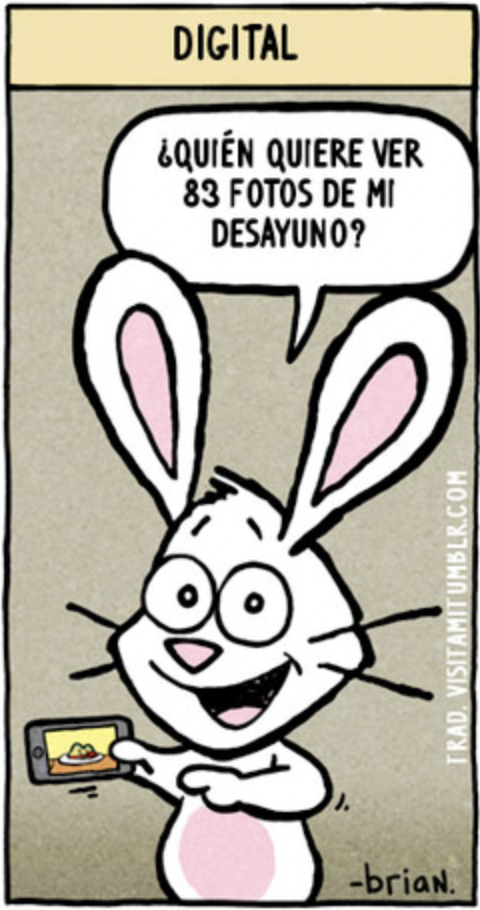
\includegraphics[scale=0.43]{digital.png} 
			
			{\scriptsize Tomado de \url{https://vivianitaparrales25.files.wordpress.com/2013/05/inicio-vivi.jpg}}
		\end{minipage}
		
		% Una imagen digital es una matriz de números reales representados por un número finito de bits.
	\end{frame}
	
	%------------------------------------------------
	% Diferencias entre los tipos de imagen
	\begin{frame}
		
		\frametitle{Imagen Analógica VS Imagen Digital}
		
		\centering
		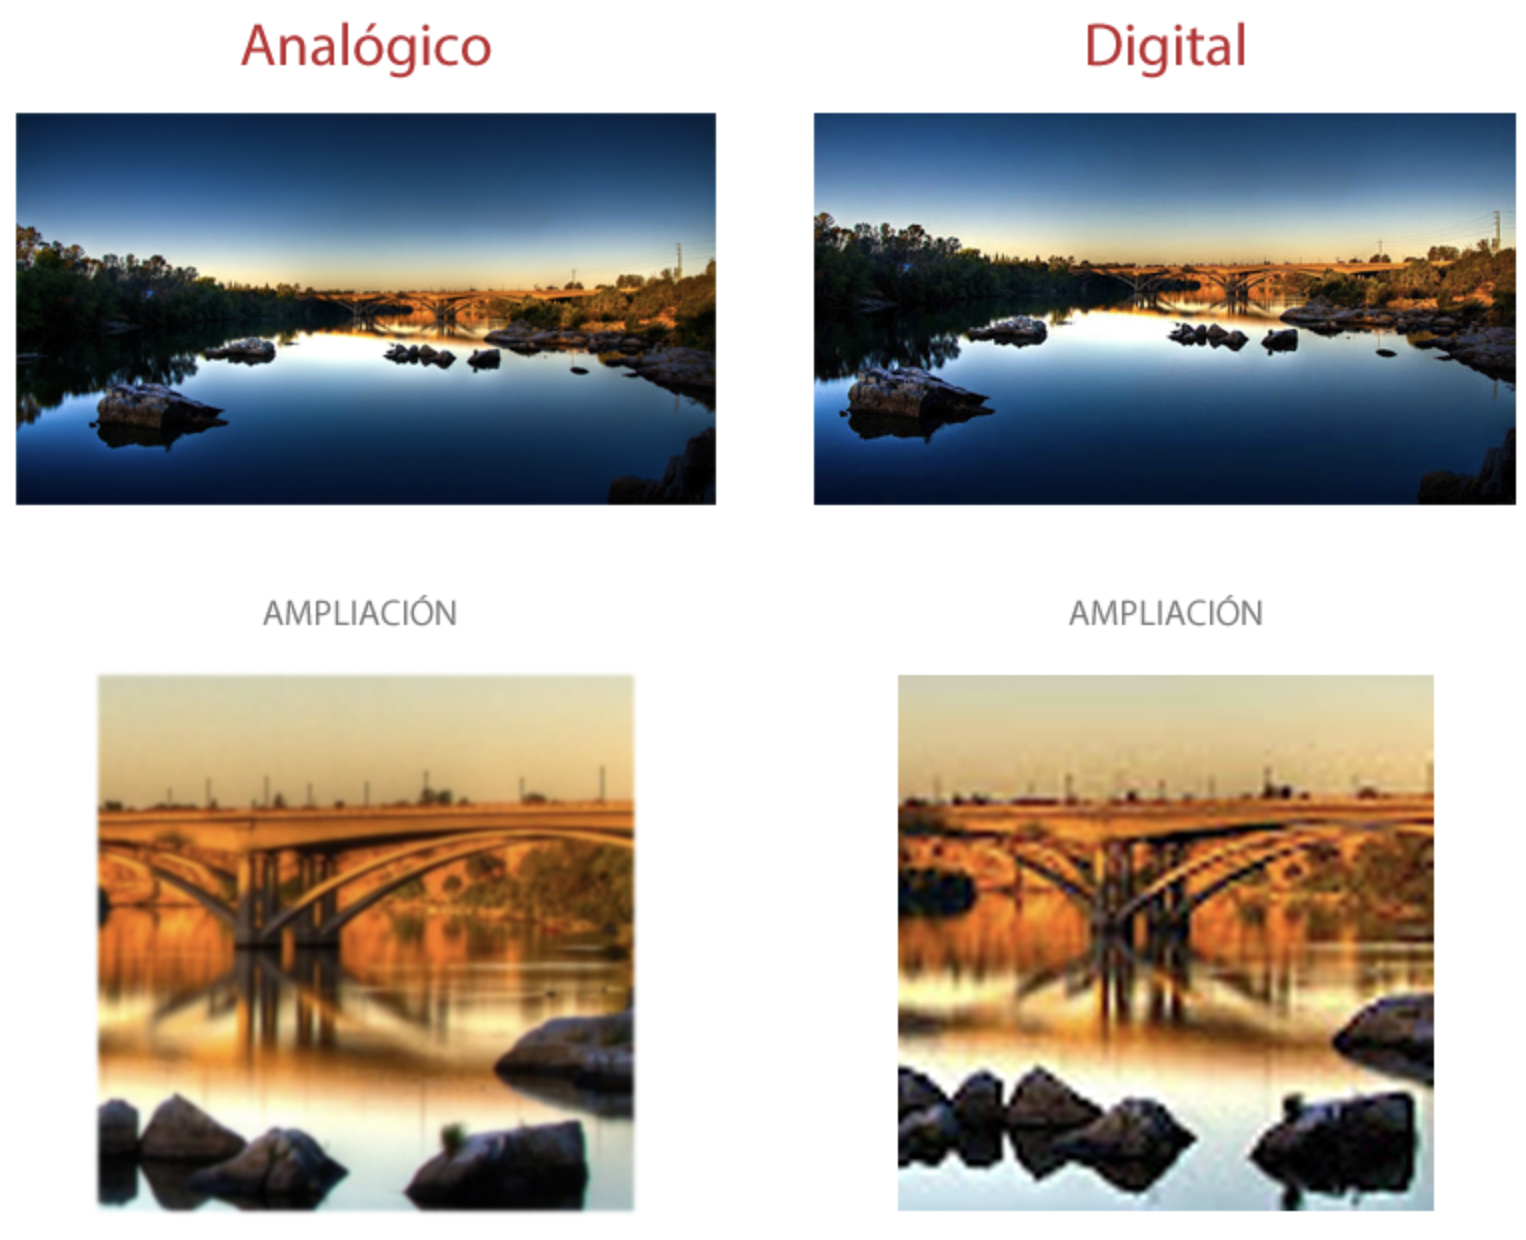
\includegraphics[scale=0.34]{diferencias.png} 
		
		{\scriptsize Tomado de \url{https://www.sound-pixel.com/blog/noticias/musica-analogica-vs-digital-aclarando-diferencias}}
		
	\end{frame}
	
	%------------------------------------------------
	% 
	\begin{frame}
		
		\frametitle{¿Recuperación de Información en imágenes?}
		
		El término Recuperación de Información sobre un conjunto de imágenes se refiere a encontrar ``esas'' imágenes que responden a la consulta efectuada por el usuario.
		
	\end{frame}
	
	
	%------------------------------------------------
	% Representación de la imagen digital
	\begin{frame}
		
		\frametitle{Representación de la imagen digital}
		
		$$f(x, y) = binario\ |\ escala\_gris\ |\ RGB$$
		
		\centering
		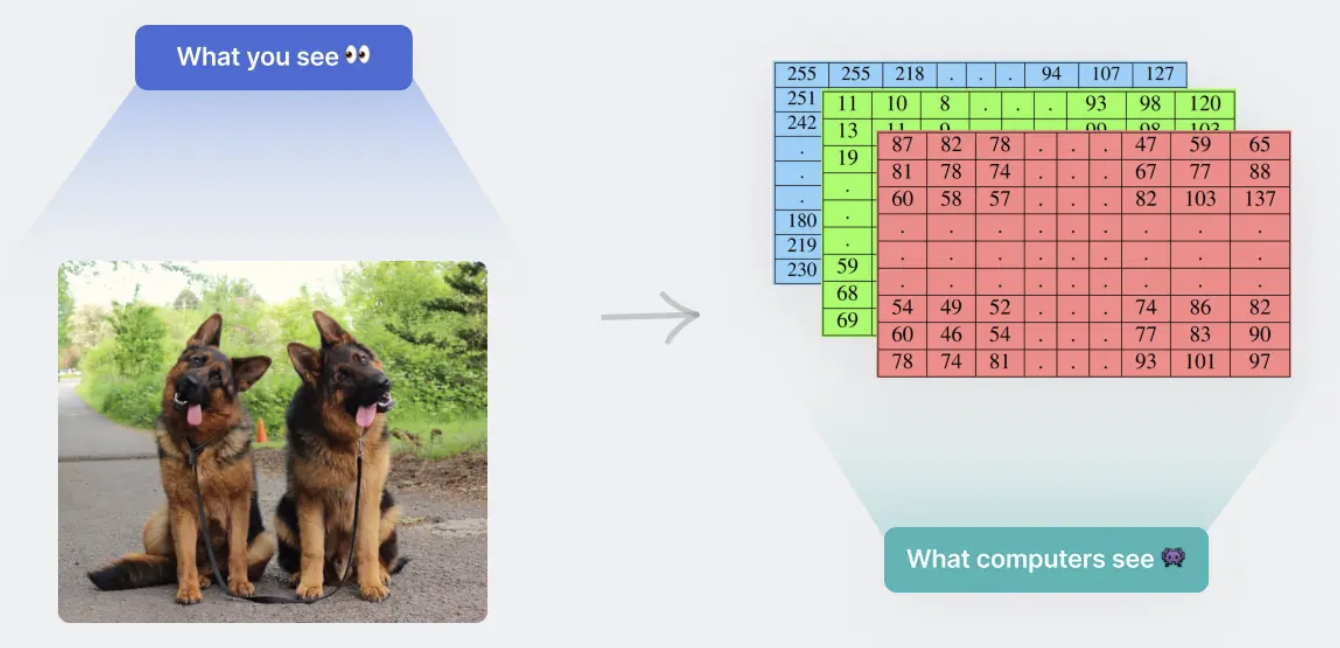
\includegraphics[scale=0.5]{representacion.png} 
			
		{\scriptsize Tomado de \url{https://www.v7labs.com/blog/image-processing-guide}}
	
	\end{frame}
	
	%------------------------------------------------
	% Representación de la imagen digital
	\begin{frame}
		
		\frametitle{Representación de la imagen digital}
		
		\noindent\begin{minipage}{.5\textwidth}
			$$f(x, y) = binario\ |\ escala\_gris\ |\ RGB$$
			$$0 \leq x < N_{filas} $$
			$$0 \leq x < M_{columnas} $$ \\[2mm]
			
			Diferentes características de la imagen, como el tamaño, el autor, la fecha u otras, son extraídas de los metadatos del fichero imagen.
			
		\end{minipage}%
		\begin{minipage}{.55\textwidth}
			\centering
			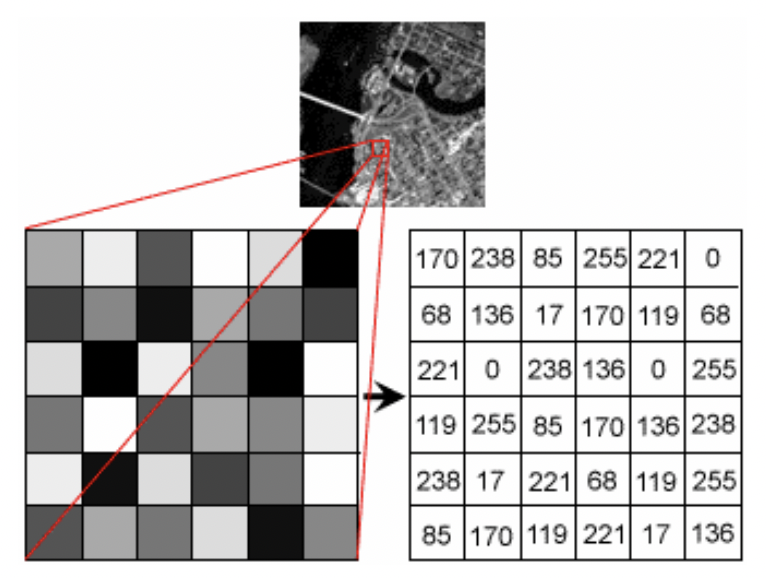
\includegraphics[scale=0.5]{coordenadas.png} 
		\end{minipage}
		
	\end{frame}
	
	%------------------------------------------------
	% Preprocesamiento en imágenes
	\begin{frame}
		
		\frametitle{Etapas del preprocesamiento en imágenes}
		
		\centering
		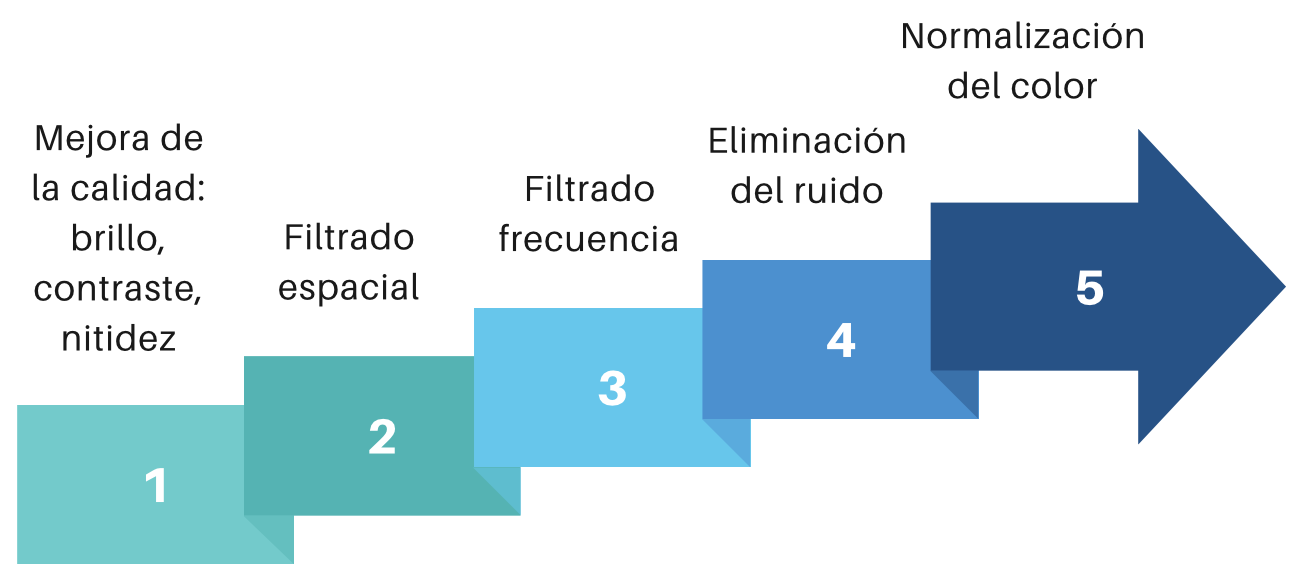
\includegraphics[scale=0.6]{preprocesamiento.png} 
		
	\end{frame}
	
	%------------------------------------------------
	% Mejora de la calidad: Brillo
	\begin{frame}
		
		\frametitle{Mejora de la calidad: Brillo}
			
		\begin{algorithmic}
			\Function{ajustar\_brillo}{imagen Image, factor\_brillo Float}
				\For{pixel $\in$ imagen}
					\State pixel $\gets$ pixel.value $*$ factor\_brillo 
				\EndFor				
			\EndFunction
		\end{algorithmic}
		
		\centering
		\vspace{1\baselineskip}
		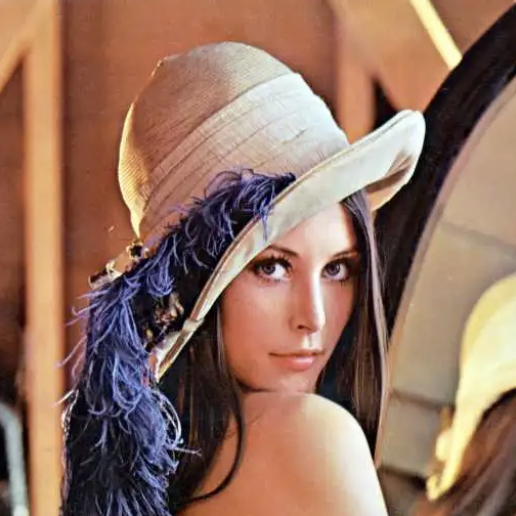
\includegraphics[scale=0.5]{lena.png} 
		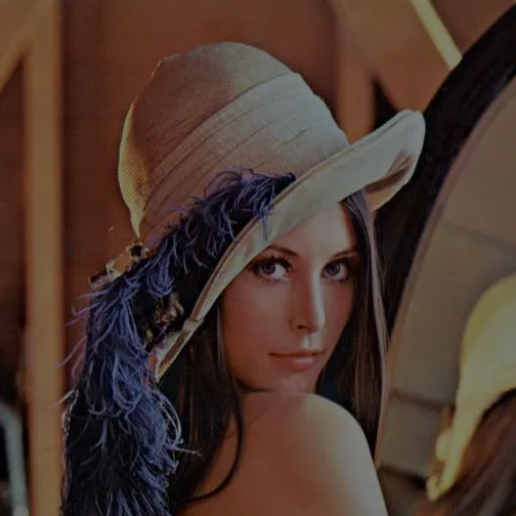
\includegraphics[scale=0.25]{lena-con-brillo.png} 
		
	\end{frame}
	
	%------------------------------------------------
	% Mejora de la calidad: Contraste
	\begin{frame}
		
		\frametitle{Mejora de la calidad: Contraste}
		
		\begin{algorithmic}
			\Function{ajustar\_nitidez}{imagen Image, factor\_contraste Float}
				\State media $\gets$ calcular\_media(imagen)
				\For{pixel $\in$ imagen}
					\State pixel $\gets ($pixel.value $-$ media$) *$ factor\_contraste $+$ media
				\EndFor				
			\EndFunction
			
			\Function{calcular\_media}{imagen Image}
			
				\Return $\frac{\sum_{pixel \in imagen} pixel.value}{imagen.ancho * imagen.alto}$
			\EndFunction
		\end{algorithmic}
		
		\centering
		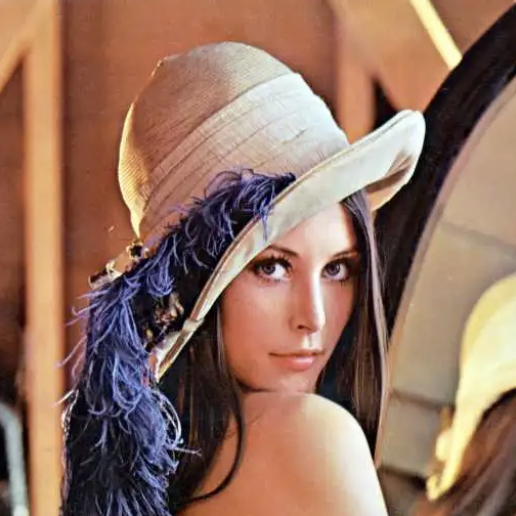
\includegraphics[scale=0.42]{lena.png} 
		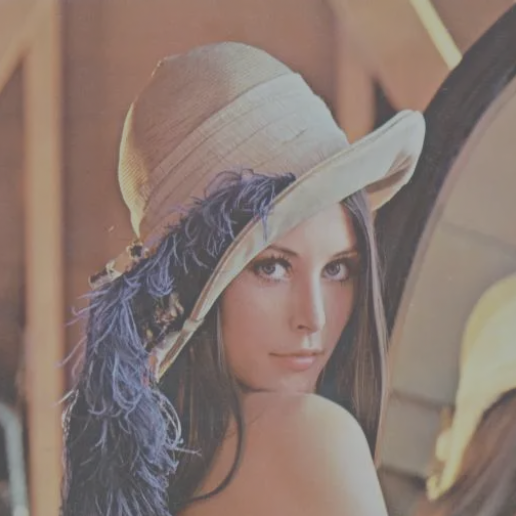
\includegraphics[scale=0.21]{lena-con-contraste.png} 
		
	\end{frame}
	
	%------------------------------------------------
	% Mejora de la calidad: Nitidez
	\begin{frame}
		
		\frametitle{Mejora de la calidad: Nitidez}
		
		\begin{algorithmic}
			\Function{ajustar\_brillo}{imagen Image, kernel Matrix}
				\For{pixel $\in$ imagen}
					\State new\_value $\gets 0$ 
					\For{np $\in$ Vencindad$($pixel, kernel$)$}
						\State new\_value $\gets$ new\_value $+($ np.value $*$ pixel.value $)$
					\EndFor
					pixe.value $\gets$ new\_value 
				\EndFor				
			\EndFunction
		\end{algorithmic}
		
		\centering
		\vspace{1\baselineskip}
		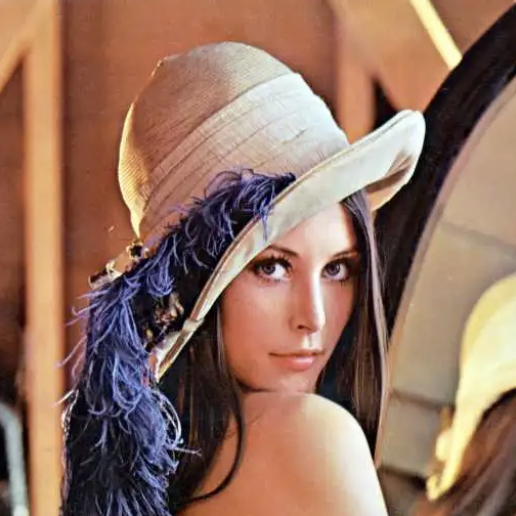
\includegraphics[scale=0.44]{lena.png} 
		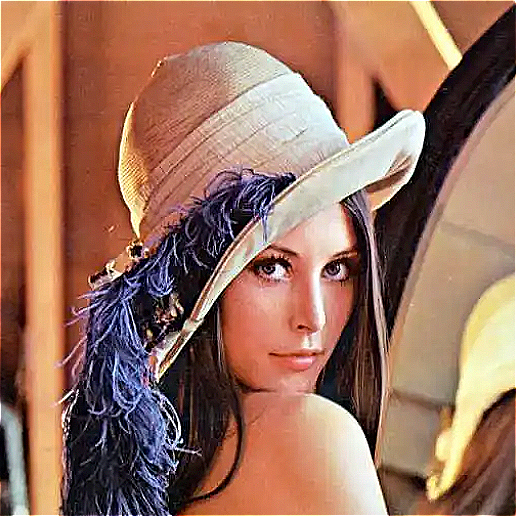
\includegraphics[scale=0.22]{lena-nitidez.png} 
		
	\end{frame}
		
	%------------------------------------------------
	% Filtrado espacial
	\begin{frame}
		
		\frametitle{Filtrado espacial}
		
		El filtrado espacial es un proceso común en el procesamiento de imágenes que implica la modificación de los valores de los píxeles de una imagen según su vecindad espacial. \\[2mm]
		
		\only<2->{El \textbf{filtrado lineal} es un tipo de filtrado espacial y se obtiene mediante una \textbf{convolución}.\\[2mm]}
		
		\only<2>{\textcolor{purple}{¿Qué es una convolución?}}
		
		\only<3->{La convolución es una operación de vecindad en la que cada píxel de salida es la suma ponderada de los píxeles de entrada vecinos. La matriz de pesos se llama núcleo de convolución o filtro.}
		
	\end{frame}
	
	%------------------------------------------------
	% Filtrado espacial
	\begin{frame}
		
		\frametitle{Algoritmo para el filtrado lineal}
		
		\begin{algorithmic}
			\Function{filtro\_lineal}{imagen Image, kernel Matrix}
			\State girar el kernel $180^\degree$
			\For{(x, y) $\in$ imagen.dimesión()}
				\State $pixel_{x,y} = \sum_{s=-a}^{b} \sum_{t=-b}^{b} kernel_{s, t}*imagen_{x+s, y+t}$
			\EndFor
			\EndFunction
		\end{algorithmic}
		
		
		\begin{minipage}{.4\textwidth}
			\centering	
			\[
			imagen=
			\left[ {\begin{array}{ccccc}
					17 &24 &  1 &  8 & 15 \\
					23 &  5 & 7 & 14 & 16 \\
					4 & 6 & 13 & 20 & 22 \\
					10 & 12 & 19 & 21 & 3 \\
					11 & 18 & 25 & 2 & 9 \\
			\end{array} } \right]
			\]
		\end{minipage}%
		\begin{minipage}{.25\textwidth}
			\centering	
			\only<1>{\[
			kernel=
			\left[ {\begin{array}{ccccc}
					8 & 1 & 6 \\
					3 & 5 & 7 \\
					4 & 9 & 2 \\
			\end{array} } \right]
			\]}
			\only<2->{\[
			kernel=
			\left[ {\begin{array}{ccccc}
					2 & 9 & 4 \\
					7 & 5 & 3 \\
					6 & 1 & 8 
			\end{array} } \right]
			\]}
		\end{minipage}%
		\begin{minipage}{.4\textwidth}
			\centering	
			\only<3->{\[
			\left[ {\begin{array}{ccccc}
					17 &24 &  1^2 &  8^9 & 15^4 \\
					23 &  5 & 7^7 & 14^5 & 16^3 \\
					4 & 6 & 13^6 & 20^1 & 22^8 \\
					10 & 12 & 19 & 21 & 3 \\
					11 & 18 & 25 & 2 & 9 \\
			\end{array} } \right]
			\]
			
			imagen[1, 3] = 275}
		\end{minipage}
		
	\end{frame}
	
	%------------------------------------------------
	% Filtrado frecuencial
	\begin{frame}
		
		\frametitle{Filtrado frecuencial}
		
		El filtrado en el dominio de la frecuencia es una técnica para realizar operaciones como el suavizado, la mejora de bordes y la eliminación de ruido. \\[2mm]
		
		\pause
		La Transformada Discreta de Fourier (TDF) es un método utilizado para filtrar frecuencia y se describe como
		$$F(u, v) = \frac{1}{M*N} \sum_{x=0}^{M-1} \sum_{y=0}^{N-1} imagen(x,y) * e^{-j2\pi(\frac{ux}{M} + \frac{vy}{N})}$$
		donde $M$ representa la cantidad de columnas y $N$ las filas. \\[2mm]
		
		\pause
		El rango del espectro de Fourier de una imagen generalmente es mucho mayor que el que puede reproducir una pantalla. Para ello, se escala el resultado como 
		$$D(u,v)=c\log(1+|F(u,v)|)$$
		
	\end{frame}
	
	%------------------------------------------------
	% Ejmeplo de aplicar TDF
	\begin{frame}
		
		\frametitle{Ejemplo de aplicar TDF}
		
		\centering
		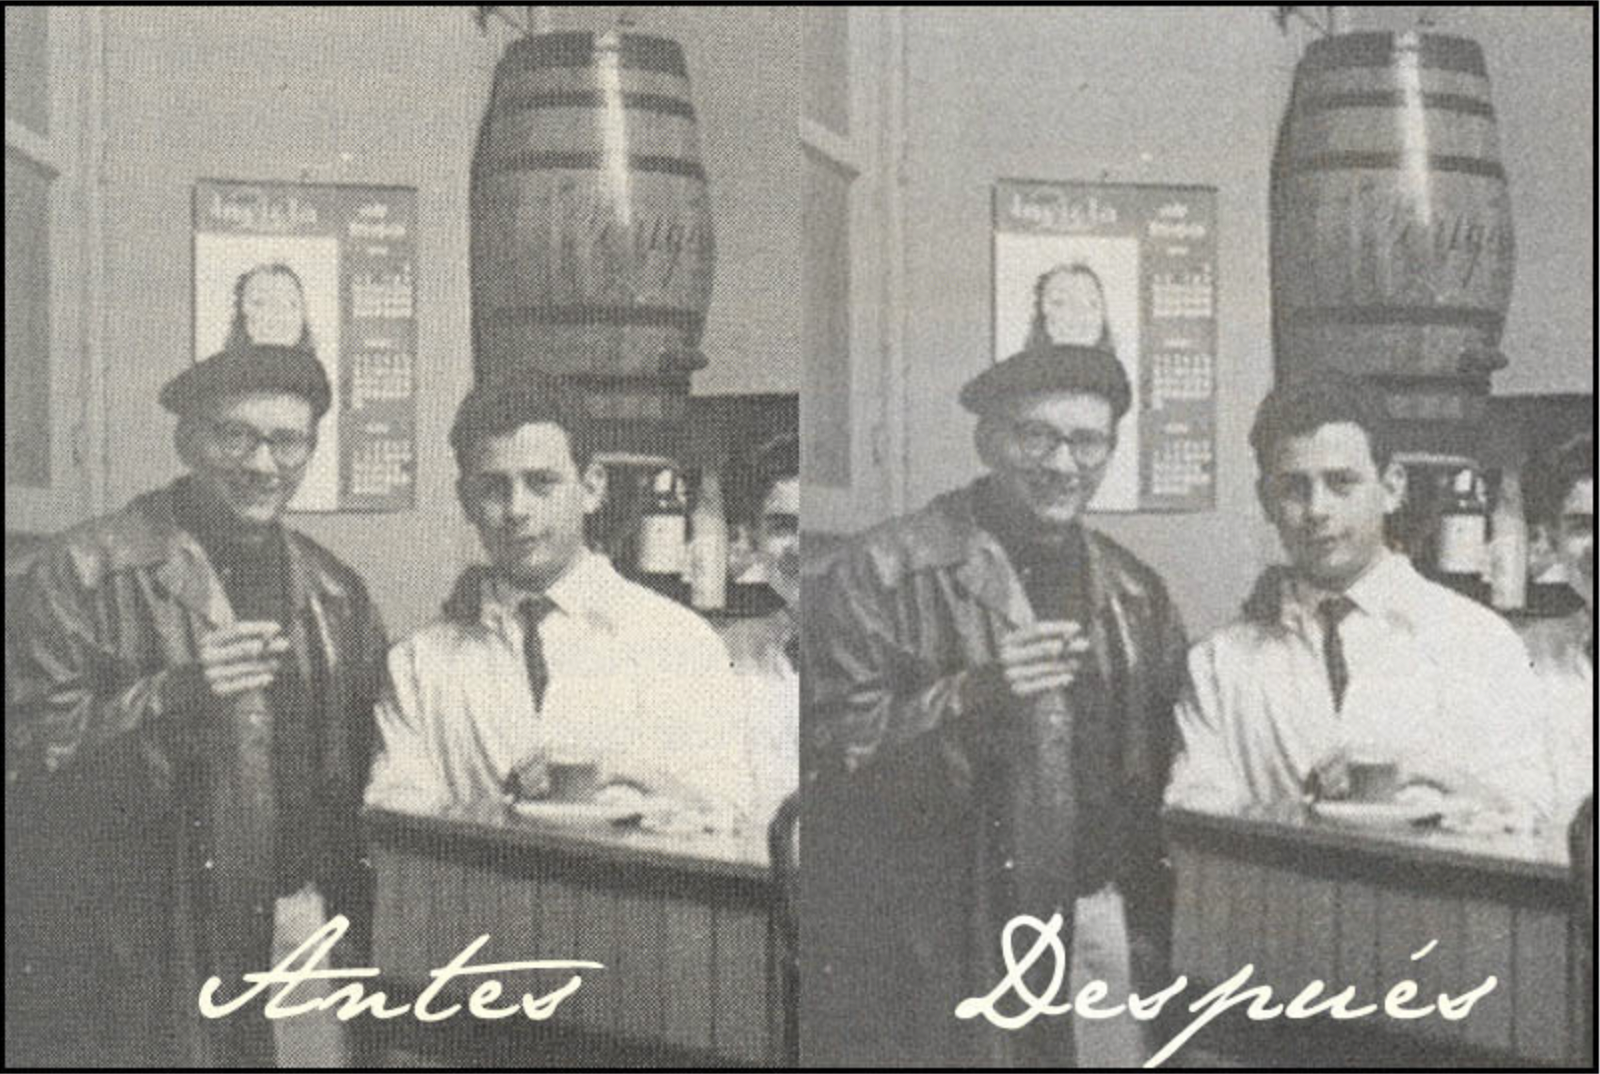
\includegraphics[scale=0.38]{tdf.png} 
		
		{\scriptsize Tomado de \url{https://visionartificialparatodos.wordpress.com/2011/01/19/tratamiento-de-imagen-ii-eliminacion-de-ruido/}}
		
	\end{frame}
	
	%------------------------------------------------
	% 
	\begin{frame}
		
		\frametitle{Eliminación de ruido}
		
		Entiéndase por \textbf{ruido} como información innecesaria, mezclada con el contenido de la imagen. Se puede expresar como 
		$$\forall pixel_{x,y} \in image, pixel_{x, y} = s_{x,y} + n_{x,y}$$
		donde $s$ es la imagen original y $n$ el ruido aplicado. \\[2mm]
		
		E]liminar este tipo de contenido sin perder la información de la imagen es una tarea complicada. \\[3mm]
		
		\pause
		Algunos algoritmos usados son: \\[2mm]
		
		\begin{minipage}{.4\textwidth}
			\begin{itemize}
				\item Filtro de Media 
				\item Filtro de Mediana
				\item Filtro Gaussiano
				\item Filtro Bilateral
			\end{itemize}
		\end{minipage}%
		\noindent\begin{minipage}{.45\textwidth}
			\begin{itemize}
				\item Filtro de Wiener
				\item Filtro de Orden de Mediana Adaptativo
				\item Filtrado en el Dominio de la Frecuencia
				\item Filtrado No Local
			\end{itemize}
		\end{minipage}%
		
	\end{frame}
	
	%------------------------------------------------
	% 
	\begin{frame}
		
		\frametitle{Algunos ejemplos de ruido}
		
		\centering
		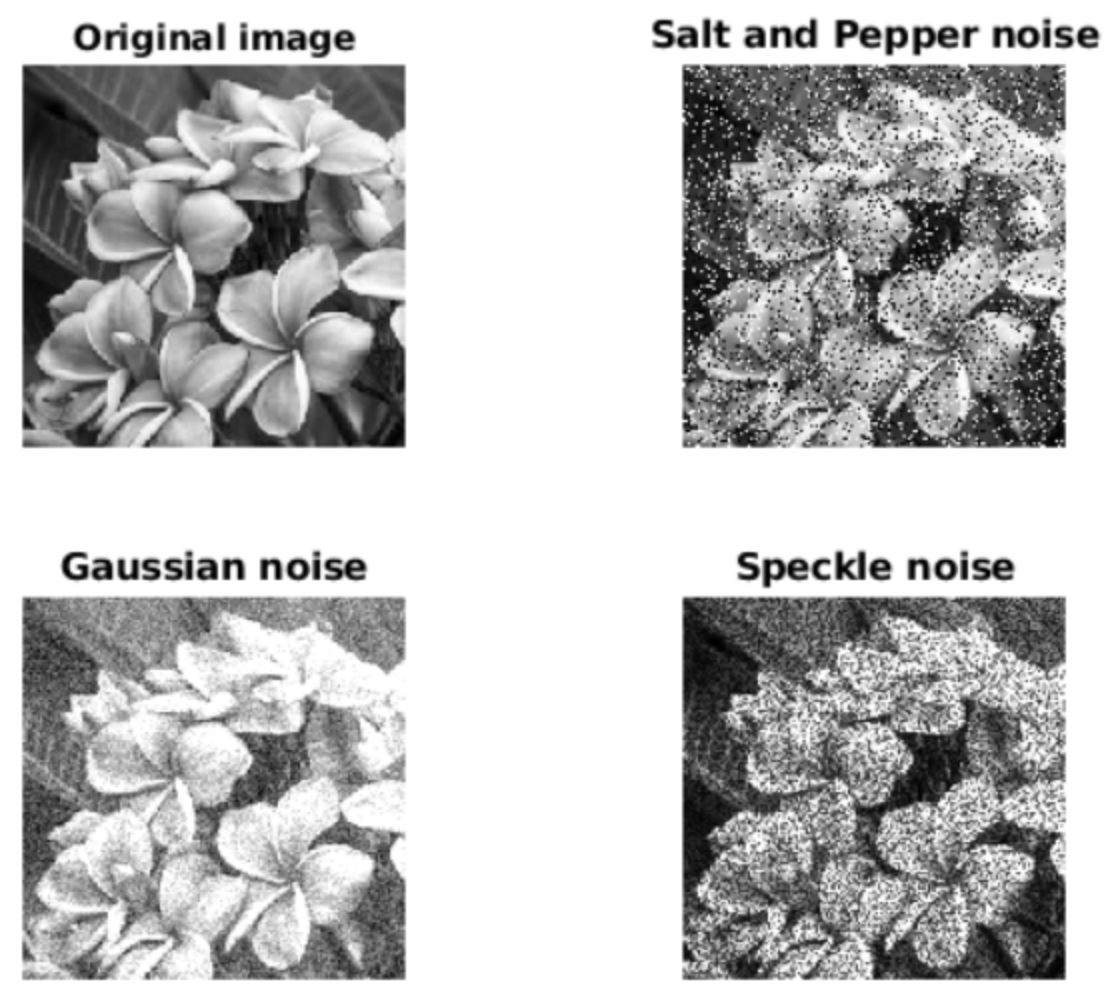
\includegraphics[scale=0.4]{ruido.png}
		
		%{\scriptsize Tomado de \url{https://www.geeksforgeeks.org/noise-addition-using-in-built-matlab-function/}}
		
		%El ruido gaussiano es ruido estadístico con una función de densidad de probabilidad (PDF) igual a la distribución normal. El ruido gaussiano tiene una distribución uniforme en toda la señal.
		
		%% Se manifiesta como píxeles blancos y negros que aparecen a intervalos aleatorios. Los errores en la transferencia de datos provocan la aparición de esta forma de ruido. Los valores a y b en el ruido de sal y pimienta son diferentes. Cada uno tiene una probabilidad de menos de 0,1 en promedio. Los píxeles corruptos se establecen alternativamente en el valor mínimo y máximo, dando a la imagen una apariencia de "sal y pimienta"
		
		%El ruido moteado es un ruido multiplicativo. En los exámenes de diagnóstico, esto reduce la calidad de la imagen al darles una apariencia de onda retrodispersada causada por muchos reflejos microscópicos dispersos que fluyen a través de los órganos internos. Esto hace que al observador le resulte más difícil distinguir los detalles finos de las imágenes. 
		
	\end{frame}
	
	%------------------------------------------------
	% Normalización y representacieon del color
	\begin{frame}
		
		\frametitle{Normalización y representación del color}
		
		\begin{itemize}
			\item Modelo RGB
			\begin{itemize}
				\item Representa cada píxel como una combinación de los componentes: rojo, verde y azul
			\end{itemize}
			
			\vspace{2\baselineskip}
			
			\item Modelo Lab
			\begin{itemize}
				\item La componente L representa la luminosidad, mientras que las componentes a y b representan los ejes de color
			\end{itemize}
		\end{itemize}
		
	\end{frame}
		
	%------------------------------------------------
	% Motivación
	\begin{frame}
		
		\frametitle{¿Qué animal se muestra?}
		
		\centering
		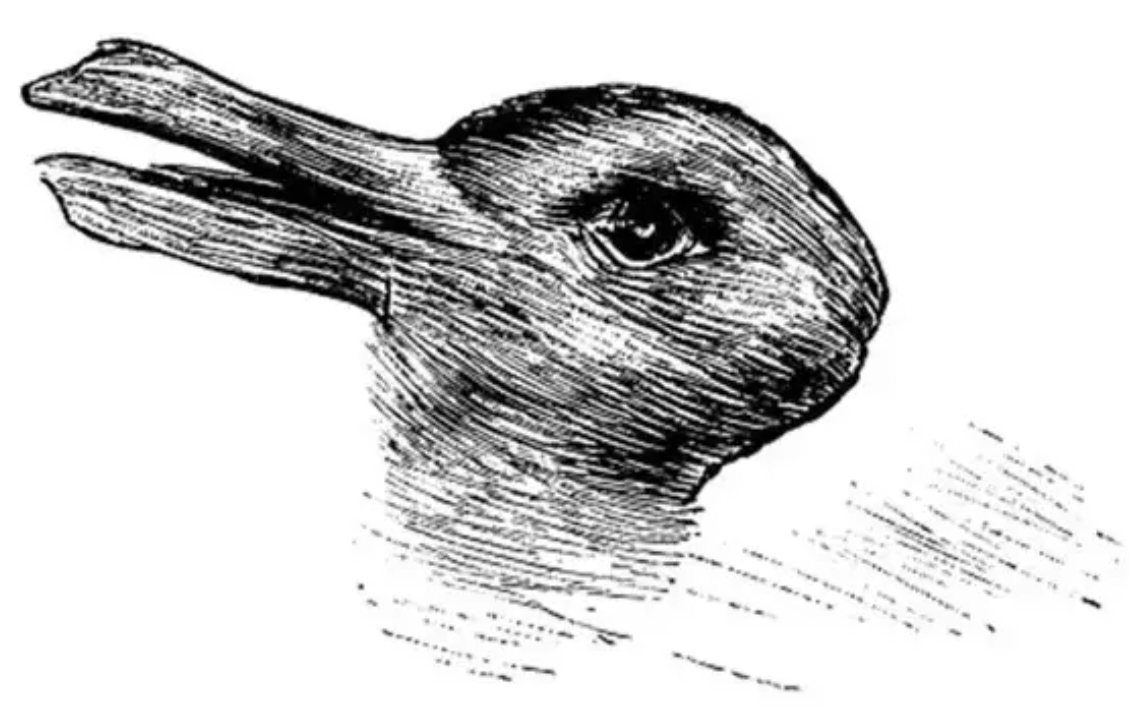
\includegraphics[scale=0.45]{pato-conejo.png} 
		
		{\scriptsize Tomado de \url{https://www.buzzfeed.com/sarahaspler/ambiguous-image-poll}}
		
		\vspace{1\baselineskip}
		\pause 
		\textcolor{purple}{¿Un pato o un conejo?}
		
		\pause 
		\textcolor{purple}{¿Qué determina el animal?}
		 
	\end{frame}
	
	%------------------------------------------------
	% Extracción de características
	\begin{frame}
		
		\frametitle{Extracción de características}
		
		\begin{alertblock}{}
			Proceso de identificar y cuantificar las propiedades visuales distintivas de una imagen que son relevantes para una tarea específica.
		\end{alertblock}
		
		\vspace{1\baselineskip}
		
		\begin{itemize}
			\item Las características pueden ser patrones, texturas, colores, formas, bordes u otros atributos visuales que son útiles para describir y distinguir objetos o regiones en una imagen.
			
			\item La extracción de características reduce la complejidad de la imagen, manteniendo la información esencial.
			
		\end{itemize}
			
	\end{frame}
	
	%------------------------------------------------
	% Descriptor de textura
	\begin{frame}
		
		\frametitle{Descriptor de textura}
		
		\begin{alertblock}{}
			Función de la variación espacial de la intensidad del brillo de los píxeles. Por tanto, la textura es un término considerado para definir objetos o conceptos de una imagen determinada.
		\end{alertblock}
		
		\pause
		\vspace{1\baselineskip}
		\centering
		\begin{forest}
			for tree={grow'=south, anchor=north}
			[ Categorías, 
			[Basado en transformaciones]
			[Estructurales]
			[Basado en modelos]
			[Estadísticos,
			[Características del histograma]
			] 
			]
		\end{forest}\\[2mm]
		
		%Existen subcategorías por cada categoría.
		
	\end{frame}
	
	%------------------------------------------------
	% Descriptor de textura: Histograma
	\begin{frame}
		
		\frametitle{Descriptor de textura: Histograma}
		
		\begin{itemize}
			\item Los indicadores estadísticos de primer orden se calculan directamente a partir de los niveles de gris de los píxeles de la imagen original, independientemente de la relación espacial entre ellos. 
			
			\item El histograma es una representación gráfica que muestra el contenido óptico de la imagen.
			
		\end{itemize}
		
		\pause
		\vspace{2\baselineskip}
		
		\centering
		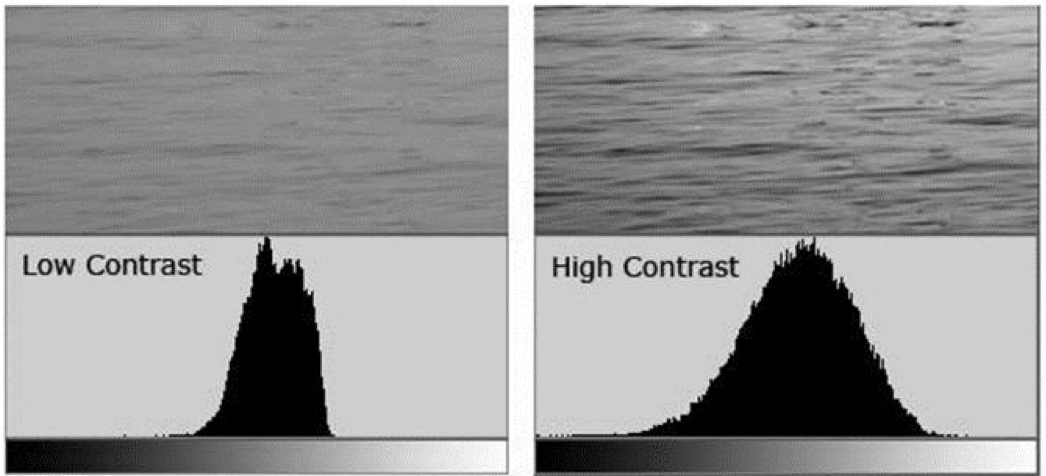
\includegraphics[scale=0.45]{textura.png} 
		
		dividir la imagen en dos
		
		{\scriptsize Tomado de \url{https://arxiv.org/pdf/1904.06554.pdf}}
		
	\end{frame}
	
	%------------------------------------------------
	% Descriptor de color
	\begin{frame}
		
		\frametitle{Descriptor de color}
		
		\begin{alertblock}{}
			Representación numérica que captura las propiedades cromáticas de una imagen. Se utilizan para caracterizar y cuantificar la distribución, la textura y la variación del color en una imagen.
		\end{alertblock}
		
		\pause
		\vspace{2\baselineskip}
		\centering
		\begin{forest}
			for tree={grow'=south, anchor=north}
			[ Categorías, 
			[Diseño de colores]
			[Estructura del color]
			[Grupo de marcos]
			[Color escalable]
			[Color dominante] 
			]
		\end{forest}
		
		
	\end{frame}
	
	%------------------------------------------------
	% Descriptor de color. Marco de color
	\begin{frame}
		
		\frametitle{Descriptor de color. Color Dominante}
		
		\begin{itemize}
			\item Parte de una imagen $[M, N]$ y devuelve una imagen de $[M/8, M/8]$
			\item Hace un cambio del espacio RGB a Lab
			\item Cada celda resultante es el valor de la representación Lab
		\end{itemize}
		
		\vspace{1\baselineskip}
		\pause
		\centering
		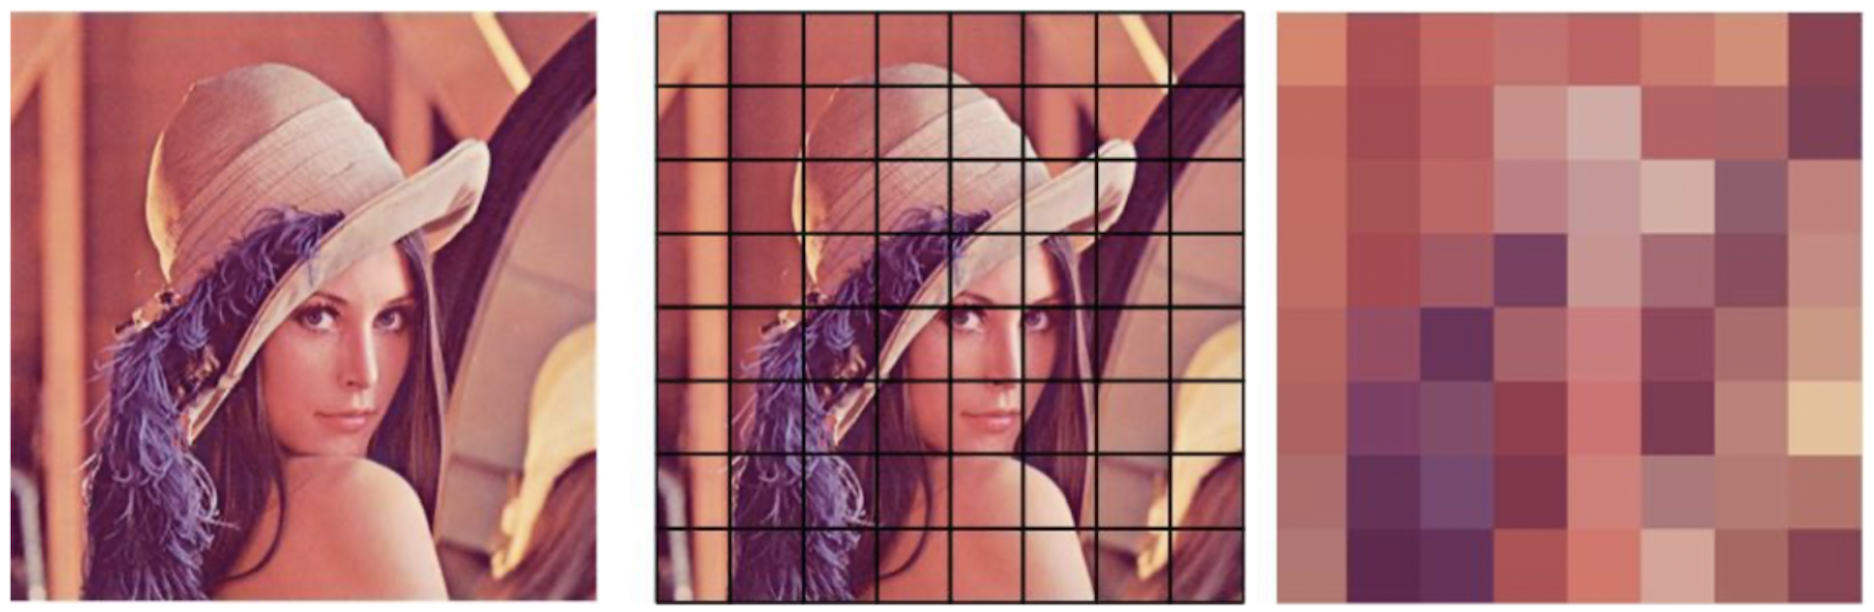
\includegraphics[scale=0.45]{dlc.png} 
		
		{\scriptsize Tomado de \url{https://core.ac.uk/reader/41812490}}
		
	\end{frame}
	
	%------------------------------------------------
	% Problemas actuales. Segmentación
	\begin{frame}
		
		\frametitle{Problemas actuales. Segmentación}
		
		\centering
		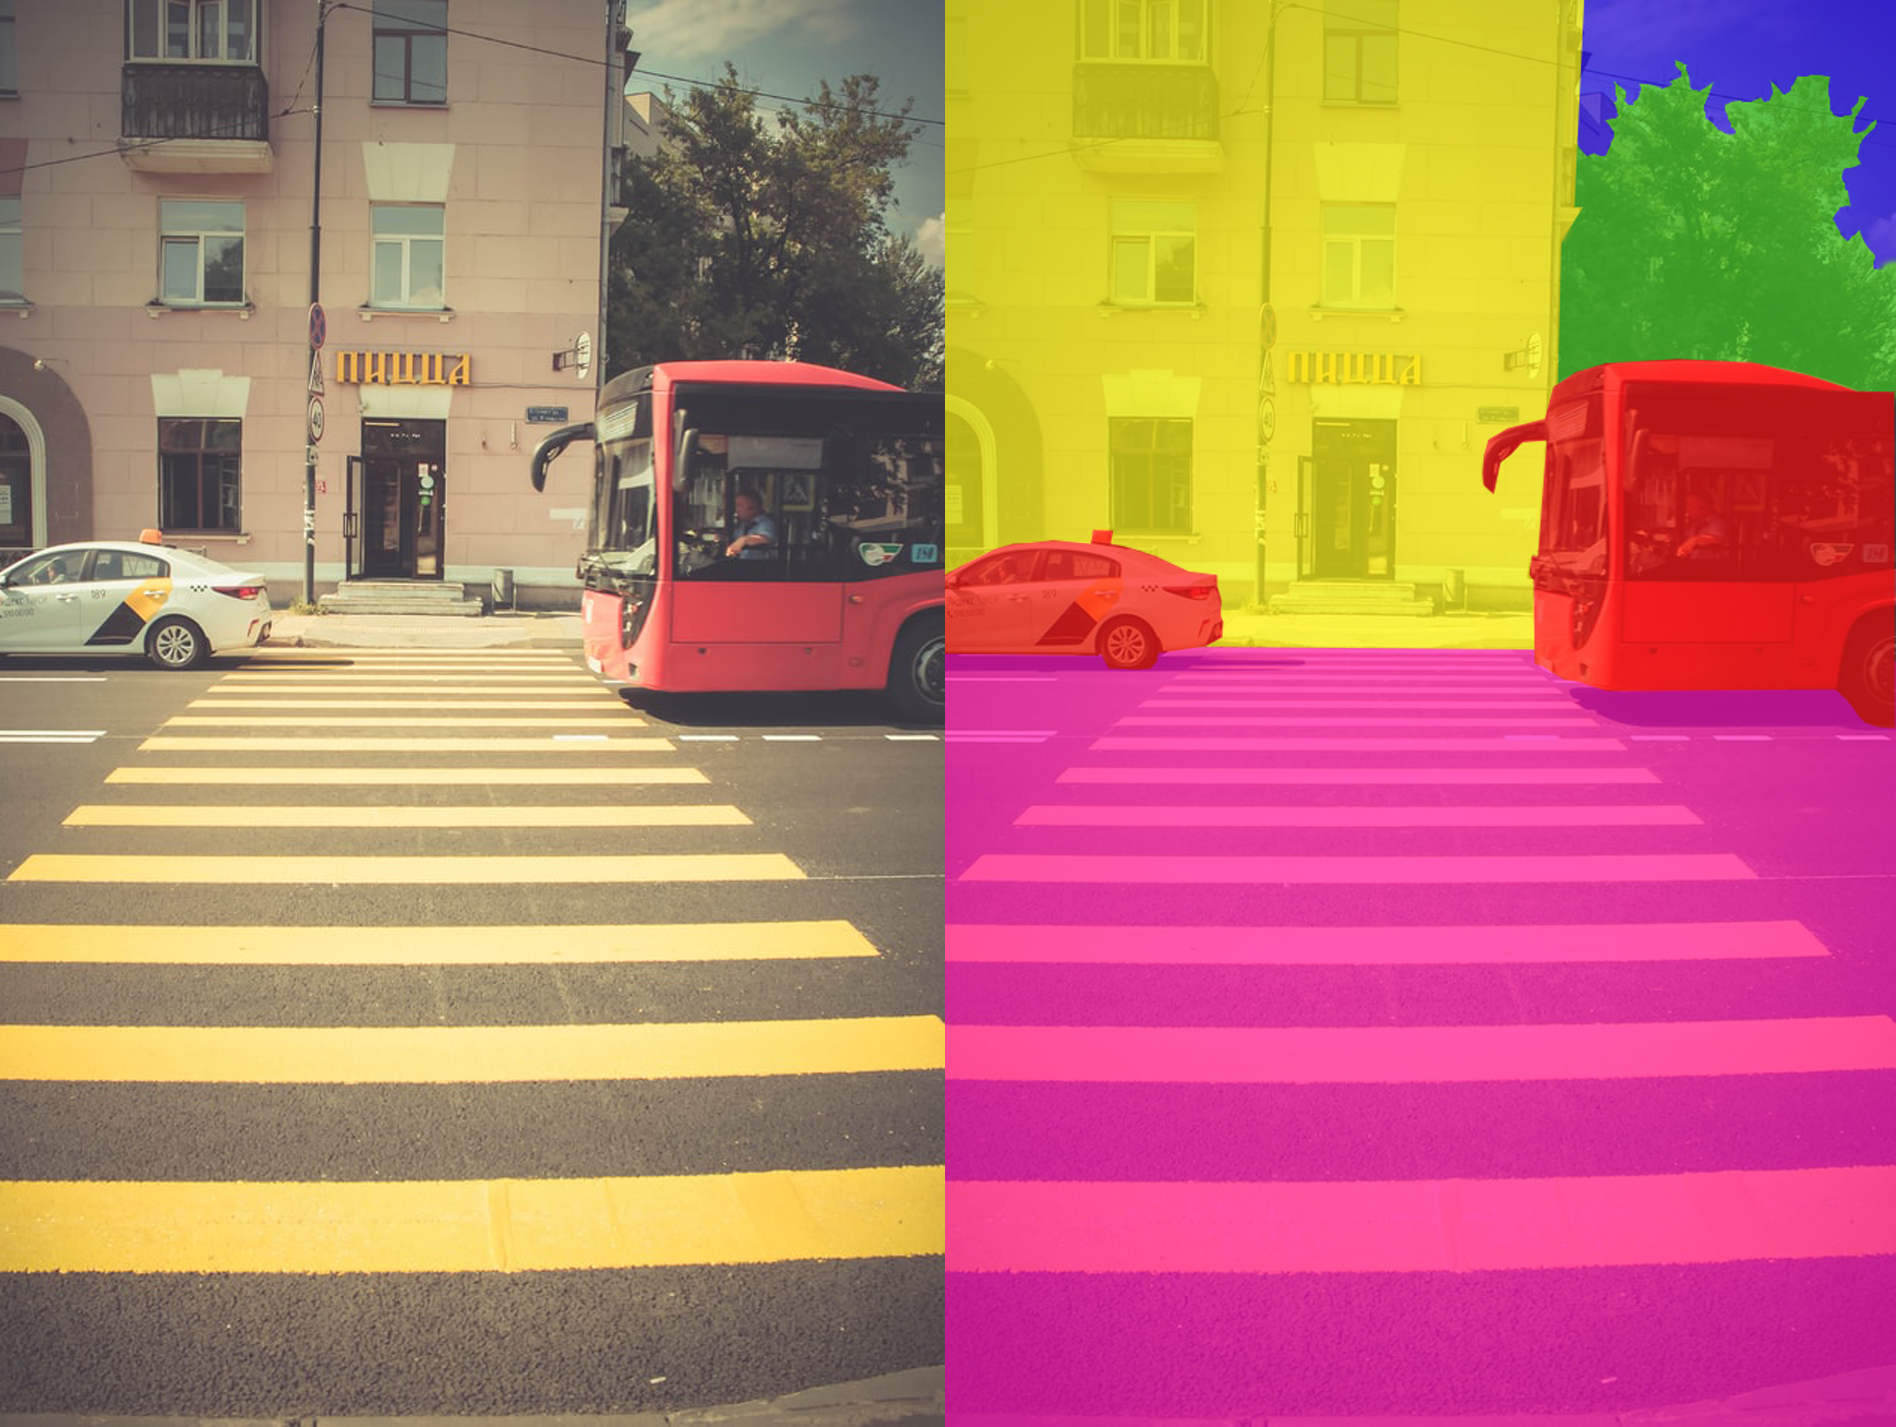
\includegraphics[scale=0.14]{segmentacion.png} 
		
		{\scriptsize Tomado de \url{https://upload.wikimedia.org/wikipedia/commons/d/d4/Image_segmentation.png}}
		
	\end{frame}
	
	%------------------------------------------------
	% Problemas actuales. Etiquetado de imagen
	\begin{frame}
		
		\frametitle{Problemas actuales. Etiquetado de imagen}
		
		\centering
		\begin{minipage}{.65\textwidth}
			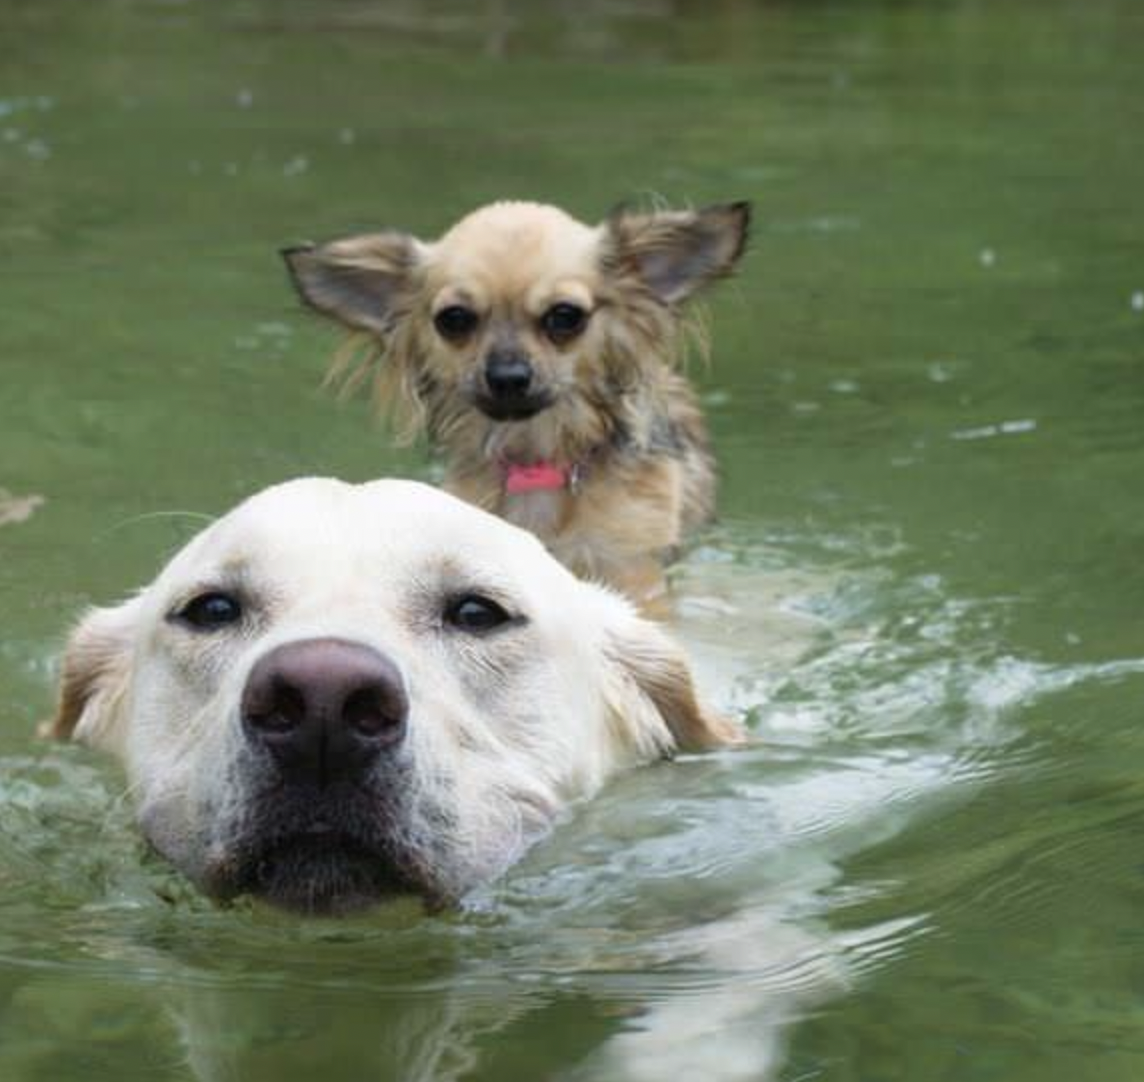
\includegraphics[scale=0.4]{perro-nadando.png} 
			
		\end{minipage}%
		\begin{minipage}{.55\textwidth}
			Describe la imagen
			
		\end{minipage}
		
		
	\end{frame}
	
	%------------------------------------------------
	% Dudas
	
	\begin{frame}
		
		\frametitle{Dudas, preguntas, sugerencias ...}
		
		\begin{figure}[h]
			\centering
			
\includegraphics[scale=0.5]{duda.png}
		\end{figure}
		
	\end{frame}	
	
	%------------------------------------------------
	% Bibliografía
	
	\begin{frame}
		
		\frametitle{Bibliografía}
		
		\begin{itemize}
			\item \url{https://www.mathworks.com/help/images/what-is-image-filtering-in-the-spatial-domain.html}		
			\item \url{https://alojamientos.us.es/gtocoma/pid/tema3-1.pdf}
			\item \url{https://riunet.upv.es/bitstream/handle/10251/68301/Ruiz\%20-\%20La\%20transformada\%20de\%20Fourier.\%20Aplicación\%20al\%20filtrado\%20de\%20imágenes.pdf}
			\item  \url{https://analyticsindiamag.com/a-guide-to-different-types-of-noises-and-image-denoising-methods/\#:~:text=A\%20type\%20of\%20noise\%20commonly,salt\%20pepper\%20noise\%20are\%20different.}
			\item Armi, Laleh; Fekri-Ershad, Shervan. Texture Image Analysis And Texture Classification Methods - A Review. \url{https://arxiv.org/pdf/1904.06554.pdf}
			\item \url{https://core.ac.uk/reader/41812490}
			
		\end{itemize}
		
	\end{frame}
	
	%------------------------------------------------
	% Fin
	
	\begin{frame}
		\titlepage
	\end{frame}
	
	
	
\end{document} 